\chapter{TINJAUAN PUSTAKA}
\label{chap:tinjauanpustaka}

% Ubah bagian-bagian berikut dengan isi dari tinjauan pustaka
\section{Hasil penelitian terdahulu}
\label{sec:roketluarangkasa}

\subsection{Deep Learning-Based Object Detection, Localisation and Tracking for Smart Wheelchair Healthcare Mobility}
\label{subsec:hukumnewton}

Pada 24 December 2020 telah dilakukan penelitian mengenai “	Deep Learning-Based Object Detection, Localisation and Tracking for Smart Wheelchair Healthcare Mobility” oleh Lecrosnier, L. \parencite{lecrosnier2021deep}

Penelitian ini bertujuan untuk mengembangkan Sistem Bantuan Pengemudi Lanjutan untuk kursi roda listrik pintar guna meningkatkan kemandirian orang-orang dengan disabilitas. Penelitian ini berfokus pada deteksi, lokalisisasi, dan pelacakan objek di dalam ruangan untuk kursi roda, khususnya pintu dan pegangan pintu.

Tujuan utama dari penelitian ini adalah meningkatkan kemampuan kursi roda otonom, yang memungkinkan deteksi objek-objek tersebut di sekitarnya secara tepat. Langkah pertama dalam penelitian ini adalah mengadaptasi algoritma deteksi objek YOLOv3 ke dalam kasus penggunaannya. Selanjutnya, penelitian ini menggunakan kamera Intel RealSense untuk melakukan estimasi kedalaman. Terakhir, sebagai langkah ketiga dan terakhir, penelitian ini menggunakan pendekatan pelacakan objek 3D berbasis algoritma SORT.

Untuk memvalidasi semua pengembangan tersebut, penelitian dilakukan dengan melakukan berbagai eksperimen di lingkungan dalam yang terkontrol. Deteksi, estimasi jarak, dan pelacakan objek diuji menggunakan dataset yang disiapkan sendiri, yang mencakup pintu dan pegangan pintu. Dengan demikian, penelitian ini bertujuan untuk meningkatkan kemampuan kursi roda pintar dalam memahami dan berinteraksi dengan lingkungannya, khususnya dalam mengenali objek-objek penting seperti pintu dan pegangannya. \parencite{lecrosnier2021deep}

\subsection{Deteksi Objek Menggunakan YOLOv3 Untuk Keamanan Pada Pergerakan Kursi Roda Elektrik}
\label{p}

Pada 12 Desember 2022 telah dilakukan penelitian mengenai “Deteksi Objek Menggunakan YOLOv3 Untuk Keamanan Pada Pergerakan Kursi Roda Elektrik”  oleh Wahyu Krisna Wijaya dan I Komang Somawirata. \parencite{wijaya2022deteksi}

Penelitian ini bertujuan untuk mengembangkan sistem pengolahan citra menggunakan algoritma You Only Look Once (YOLO), untuk meningkatkan keamanan pergerakan kursi roda elektrik. Sistem ini dirancang untuk mendeteksi objek di depan kursi roda, termasuk halangan di permukaan jalan dan objek yang dapat menghalangi pergerakan kursi roda tersebut contohnya seperti meja, kursi dan barang - barang yang ada di lingkungan sehari-hari.

Dengan menggunakan teknologi pengolahan citra, sistem ini dapat secara otomatis mendeteksi objek-objek tersebut saat kursi roda bergerak. Hasil pendeteksian tersebut kemudian ditampilkan pada layar monitor di depan pengemudi, memungkinkan mereka untuk merespons dengan cepat terhadap potensi bahaya di jalur perjalanan.

Tujuan utama dari penelitian ini adalah untuk meningkatkan keamanan pengguna kursi roda elektrik dengan fokus pada pendeteksian objek di sekitar kursi roda. Dengan demikian, sistem ini memberikan kontribusi dalam mendukung sistem keamanan kursi roda elektrik, khususnya dalam menghadapi situasi di mana ada halangan di depan atau di sekitar kursi roda yang dapat membahayakan pengguna.

\subsection{Deteksi Plat Nama Ruangan untuk Kendali Kursi Roda Pintar menggunakan YOLOv5 dan EasyOCR berbasis TX2}

Pada 2 Maret 2023 telah dilakukan penelitian mengenai "Deteksi Plat Nama Ruangan untuk Kendali Kursi Roda Pintar menggunakan YOLOv5 dan EasyOCR berbasis TX2" oleh Muhammad Fadhel Haidar dan Fitri Utaminingrum.

Penelitian ini bertujuan untuk Mengembangankan sistem deteksi nama ruangan otomatis untuk kursi roda pintar untuk membantu penyandang disabilitas mendapatkan mobilitas yang lebih baik. Menggunakan kamera, sistem ini dapat mengenali plat nama ruangan melalui metode YOLOv5 dan EasyOCR.

Penelitian ini menunjukkan bahwa metode YOLOv5 memiliki akurasi 60\% dalam mendeteksi nama ruangan, sementara EasyOCR mencapai 100\%. Hasil ini memvalidasi kemungkinan integrasi sistem deteksi objek dan pengenalan karakter untuk meningkatkan navigasi kursi roda otonom.

Kesimpulan dari penelitian tersebut adalah bahwa sistem deteksi nama ruangan otomatis pada kursi roda pintar yang menggunakan metode YOLOv5 dan EasyOCR terbukti efektif dalam membantu navigasi penyandang disabilitas. Meskipun metode YOLOv5 menunjukkan akurasi yang lebih rendah (60\%) dibandingkan EasyOCR (100\%), integrasi kedua metode tersebut meningkatkan kemampuan kursi roda untuk bergerak secara otonom menuju tujuan yang diinginkan berdasarkan pengenalan plat nama ruangan. Ini membuka peluang untuk pengembangan lebih lanjut dalam teknologi bantu mobilitas bagi penyandang disabilitas.

\section{Object Detection}
Deteksi objek secara real-time telah muncul sebagai komponen kritis dalam berbagai aplikasi, meliputi berbagai bidang seperti kendaraan otonom, robotika, pengawasan video, dan realitas tertambah. Di antara berbagai algoritma deteksi objek, kerangka kerja YOLO (\emph{You Only Look Once}) telah menonjol karena keseimbangan kecepatan dan akurasi yang luar biasa, memungkinkan identifikasi objek yang cepat dan dapat diandalkan dalam gambar. Sejak diperkenalkan, keluarga YOLO telah berkembang melalui beberapa iterasi, setiap versi membangun atas versi sebelumnya untuk mengatasi keterbatasan dan meningkatkan kinerja.

Selain kerangka kerja YOLO, bidang deteksi objek dan pemrosesan gambar telah mengembangkan beberapa metode lain yang terkenal. Teknik seperti R-CNN (\emph{Region-based Convolutional Neural Networks}) dan penerusnya, Fast R-CNN dan Faster R-CNN, telah memainkan peran penting dalam memajukan akurasi deteksi objek. Metode ini mengandalkan proses dua tahap, di mana pencarian selektif menghasilkan usulan wilayah, dan jaringan saraf konvolusional mengklasifikasi dan menyempurnakan wilayah-wilayah ini. Pendekatan signifikan lainnya adalah Single-Shot MultiBox Detector (SSD), yang, serupa dengan YOLO, berfokus pada kecepatan dan efisiensi dengan menghilangkan kebutuhan untuk langkah usulan wilayah terpisah. Selain itu, metode seperti Mask R-NN telah memperluas kemampuan ke segmentasi instans, memungkinkan lokalizasi objek yang tepat dan segmentasi tingkat piksel. Perkembangan ini, bersama dengan lainnya seperti RetinaNet dan EfficientDet, telah secara kolektif berkontribusi pada lanskap beragam algoritma deteksi objek. Setiap metode menawarkan kompromi unik antara kecepatan, akurasi, dan kompleksitas, melayani kebutuhan aplikasi yang berbeda dan kendala komputasi.\parencite{Yolov8}

\section{YOLO (\emph{You Only Look Once})}
YOLO oleh \cite{YOLO}. Joseph Redmoon untuk pertama kalinya memperkenalkan pendekatan \emph{End to end} pada deteksi objek secara \emph{Real Time}. Nama YOLO, yang merupakan singkatan dari \emph{"You Only Look Once"} (Anda Hanya Melihat Sekali), merujuk pada kemampuannya untuk menyelesaikan tugas deteksi dengan hanya satu kali laluan jaringan, berbeda dengan pendekatan sebelumnya yang menggunakan jendela geser diikuti oleh pengklasifikasi yang harus dijalankan ratusan atau ribuan kali per gambar atau metode yang lebih canggih yang membagi tugas menjadi dua langkah, di mana langkah pertama mendeteksi kemungkinan daerah dengan objek atau proposal daerah dan langkah kedua menjalankan pengklasifikasi pada proposal tersebut. Selain itu, YOLO menggunakan keluaran yang lebih sederhana berdasarkan hanya regresi untuk memprediksi keluaran deteksi sebagai lawan dari Fast R-CNN yang menggunakan dua keluaran terpisah, sebuah klasifikasi untuk probabilitas dan regresi untuk \emph{box} koordinat\parencite{YOLO}

\subsection{YOLOv8}
YOLOv8 diluncurkan pada Januari 2023 oleh \emph{Ultralytics}, perusahaan yang mengembangkan YOLOv5. YOLOv8 menyediakan lima versi skala: YOLOv8n (nano), YOLOv8s (kecil), YOLOv8m (sedang), YOLOv8l (besar), dan YOLOv8x (ekstra besar). YOLOv8 mendukung berbagai tugas visi seperti deteksi objek, segmentasi, estimasi pose, pelacakan, dan klasifikasi.\parencite{Yolov8}

% Contoh input gambar
\begin{figure}[H]
  \centering

  % Ubah dengan nama file gambar dan ukuran yang akan digunakan
  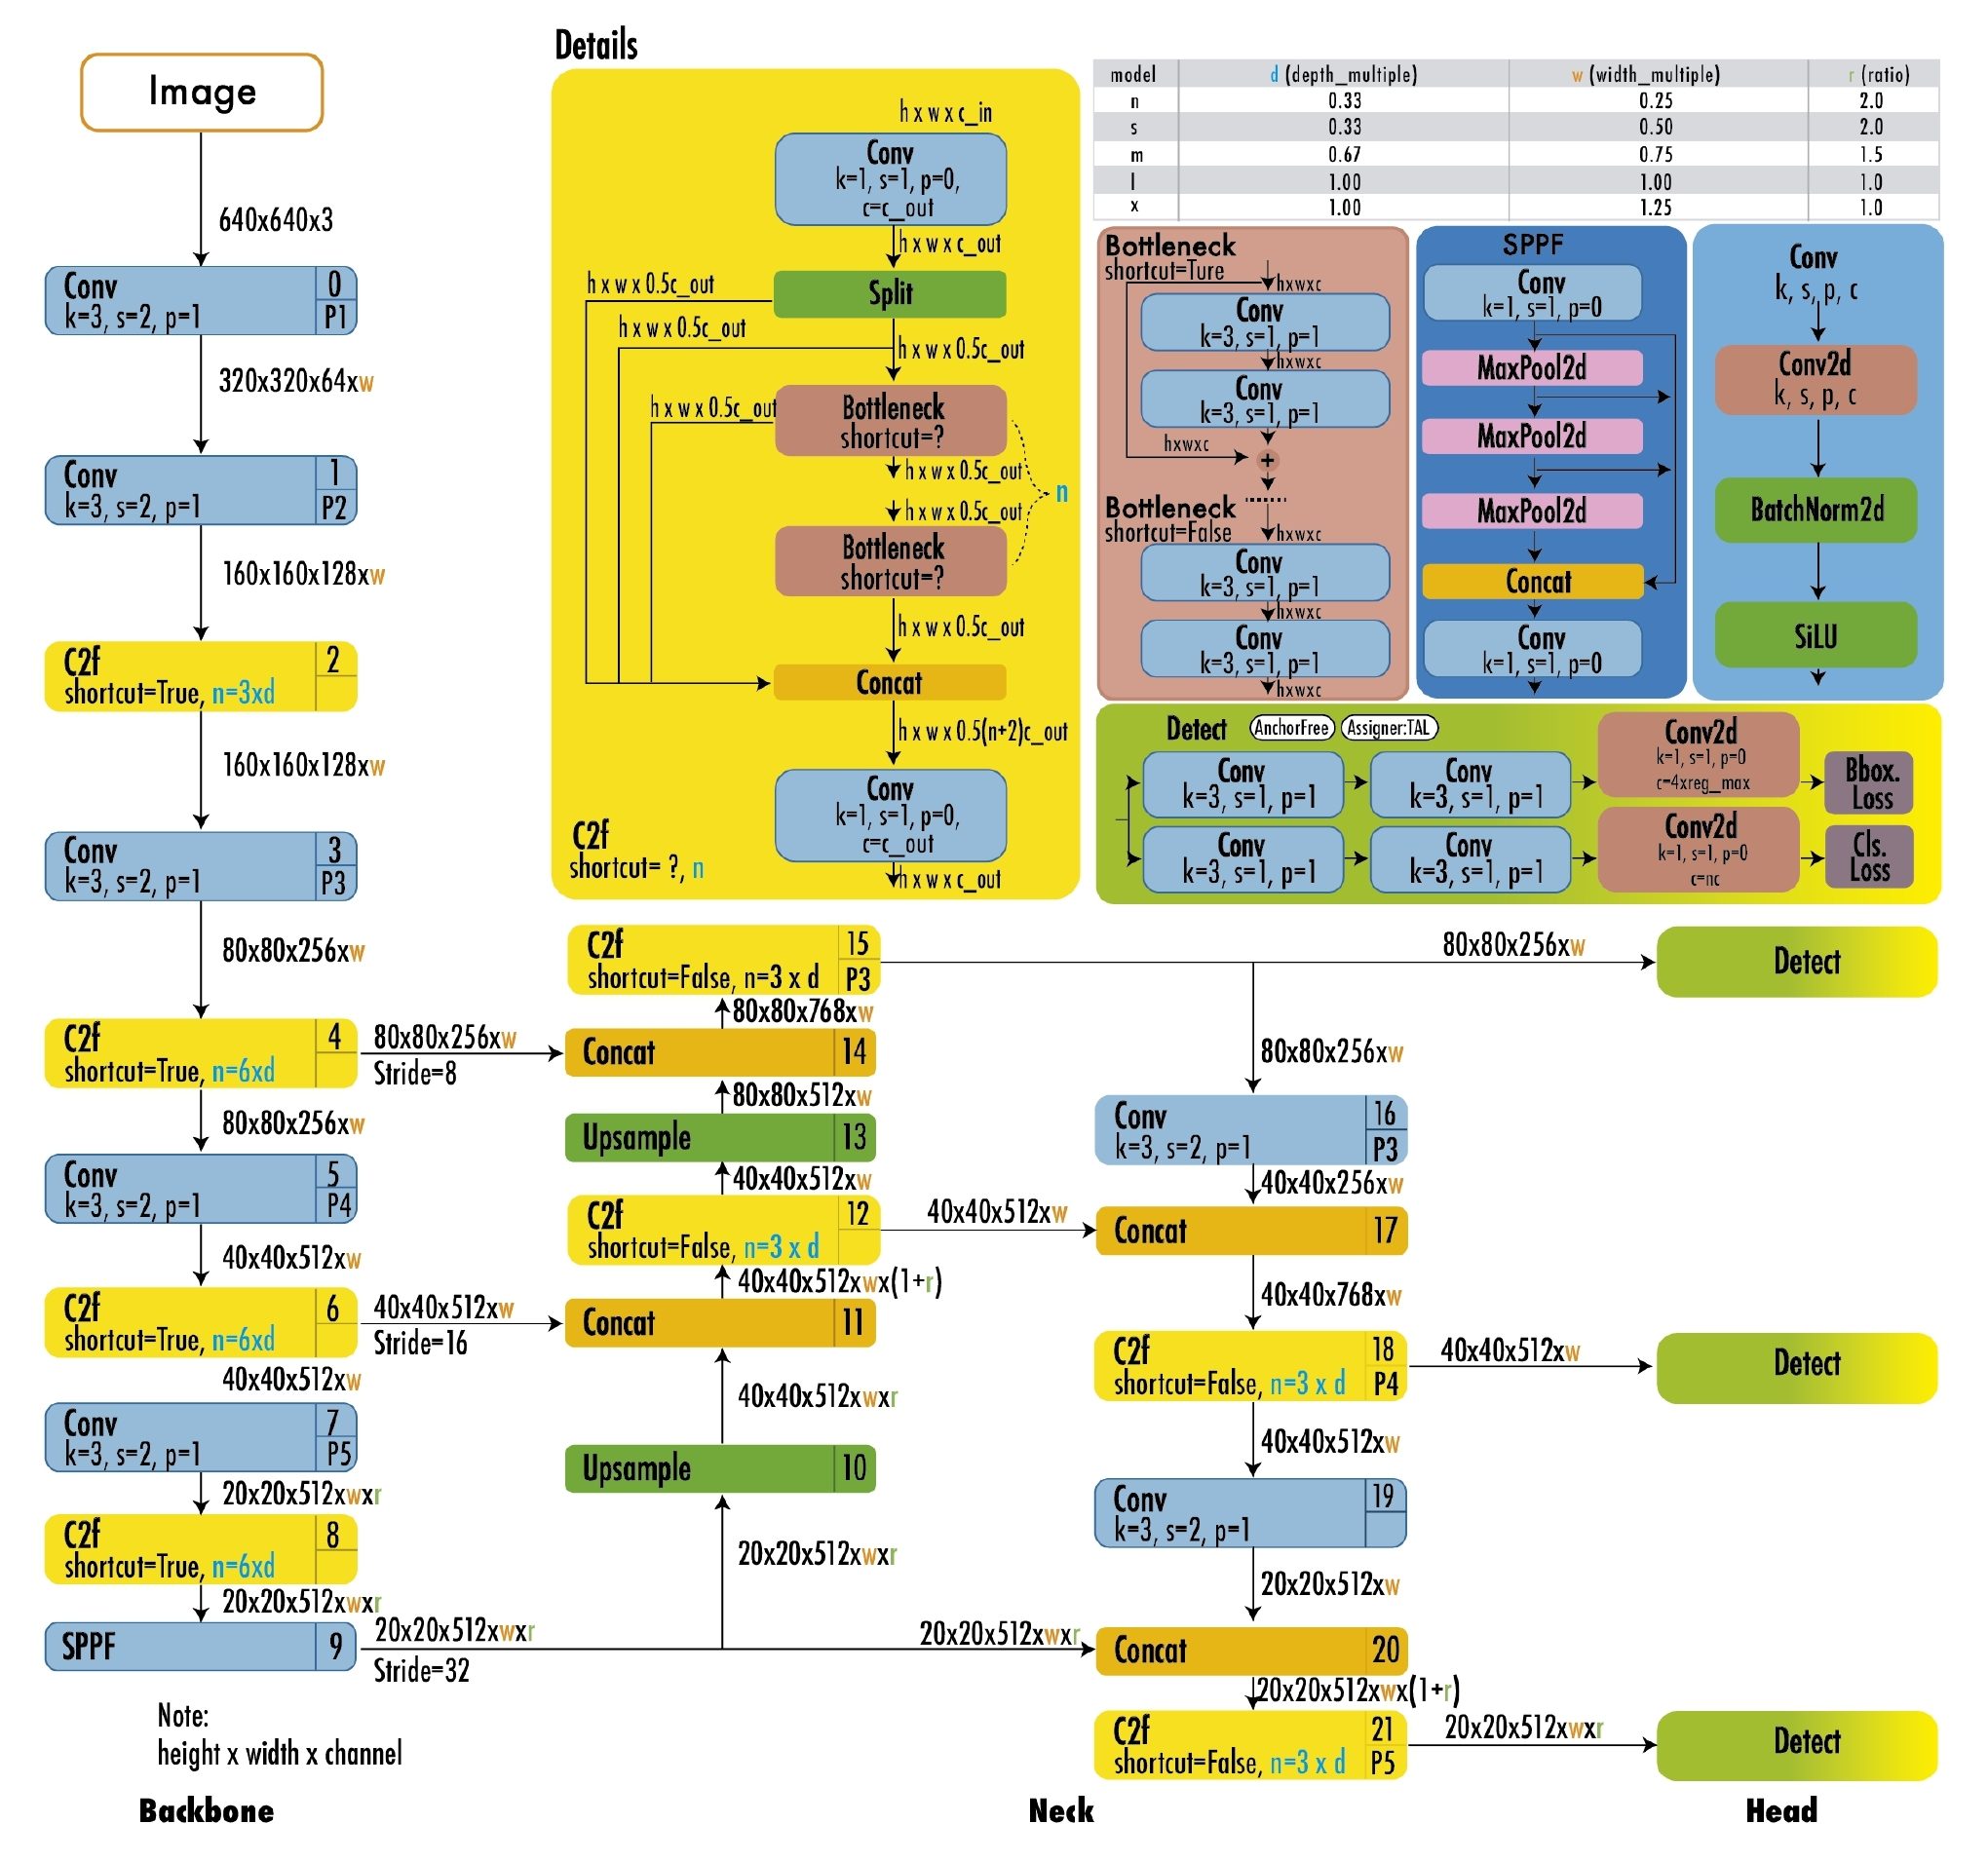
\includegraphics[scale=0.5]{gambar/YoloV8Architecture.jpg}

  % Ubah dengan keterangan gambar yang diinginkan
  \caption{Arsitektur YOLOv8.}
  \label{fig:Arsitektur Yolov8}
\end{figure}

Pada Gambar 2.1 merupakan gambar detail Arsitektur Yolov8.YOLOv8 menggunakan backbone yang serupa dengan YOLOv5 dengan beberapa perubahan pada CSPLayer, yang kini disebut modul C2f. Modul C2f (\emph{cross-stage partial bottleneck with two convolutions}) menggabungkan fitur tingkat tinggi dengan informasi kontekstual untuk meningkatkan akurasi deteksi.

YOLOv8 menggunakan model \emph{anchor-free} dengan \emph{decoupled head} untuk memproses tugas klasifikasi , dan regresi secara independen. Desain ini memungkinkan setiap cabang untuk fokus pada tugasnya dan meningkatkan akurasi model secara keseluruhan. Di output layer dari YOLOv8, mereka menggunakan fungsi aktivasi sigmoid untuk objectness score, yang mewakili probabilitas bahwa \emph{bounding box} mengandung suatu objek. Model ini menggunakan fungsi softmax untuk \emph{class probabilities}, yang mewakili probabilitas objek yang termasuk dalam setiap kelas yang mungkin.

YOLOv8 menggunakan \emph{loss functions} CIoU dan DFL untuk \emph{bounding box loss} dan \emph{binary cross-entropy} untuk \emph{classification loss}. Loss ini telah meningkatkan kinerja \emph{object detection}, terutama saat berhadapan dengan objek yang lebih kecil.

YOLOv8 juga menyediakan semantic \emph{segmentation model} yang disebut YOLOv8-Seg model. Backbone adalah CSPDarknet53 \emph{feature extractor}, diikuti oleh modul C2f bukan traditional YOLO neck architecture. Modul C2f diikuti oleh dua segmentation heads, yang belajar memprediksi semantic \emph{segmentation masks} untuk input image. Model ini memiliki \emph{detection heads} yang mirip dengan YOLOv8, terdiri dari lima detection modules dan prediction layer. YOLOv8-Seg model telah mencapai \emph{state-of-the-art results} pada berbagai \emph{object detection} dan \emph{semantic segmentation benchmarks} sambil menjaga \emph{high speed} dan efisiensi.

YOLOv8 dapat dijalankan dari \emph{command line interface} (CLI), atau juga dapat dipasang sebagai PIP package. Selain itu, dilengkapi dengan berbagai integrations untuk labeling, training, dan deploying.

Nilai Evaluasi pada MS COCO dataset test-dev 2017, YOLOv8x mencapai AP sebesar 53.9\% dengan image size 640 pixels (dibandingkan dengan 50.7\% dari YOLOv5 pada size input yang sama) dengan speed 280 FPS pada NVIDIA A100 dan TensorRT.

\section{Pose Estimation}
Estimasi pose adalah tugas menggunakan model pembelajaran mesin (\emph{ML}) untuk memperkirakan pose seseorang dari gambar atau video dengan mengestimasi lokasi spasial sendi tubuh utama (titik kunci atau \emph{keypoints}). Estimasi pose merujuk pada teknik visi komputer yang mendeteksi sosok manusia dalam gambar dan video, sehingga seseorang dapat menentukan, misalnya, di mana siku seseorang muncul dalam gambar. Penting untuk menyadari bahwa estimasi pose hanya memperkirakan di mana sendi tubuh kunci berada dan tidak mengenali siapa yang ada dalam gambar atau video.\parencite{tensorflow2015-whitepaper}

Model estimasi pose mengambil gambar kamera yang telah diproses sebagai input dan mengeluarkan informasi tentang titik kunci. Titik kunci yang terdeteksi diindeks oleh ID bagian, dengan skor kepercayaan antara 0,0 dan 1,0. Skor kepercayaan menunjukkan probabilitas bahwa titik kunci ada di posisi tersebut.\parencite{tensorflow2015-whitepaper}

\section{MediaPipe}
MediaPipe adalah kerangka kerja untuk membangun pipa yang melakukan inferensi dari data sensorik apa pun. Dengan MediaPipe, pipa persepsi dapat dibangun sebagai graf dari komponen modular, termasuk inferensi model, algoritma pengolahan media, dan transformasi data, dll. Data sensorik seperti aliran audio dan video memasuki graf, dan deskripsi yang dirasakan seperti aliran lokalizasi objek dan landmark wajah keluar dari graf. MediaPipe dirancang untuk praktisi pembelajaran mesin (ML) (\emph{machine learning}), termasuk peneliti, mahasiswa, dan pengembang perangkat lunak, yang mengimplementasikan aplikasi ML yang siap produksi, menerbitkan kode yang menyertai karya penelitian, dan membangun prototipe teknologi. Kasus penggunaan utama untuk MediaPipe adalah prototipe cepat dari pipa persepsi dengan model inferensi dan komponen yang dapat digunakan kembali lainnya. MediaPipe juga memfasilitasi penyebaran teknologi persepsi ke dalam demo dan aplikasi di berbagai platform perangkat keras yang berbeda. MediaPipe memungkinkan peningkatan bertahap pada pipa persepsi melalui bahasa konfigurasi yang kaya dan alat evaluasi. \parencite{MediaPipe}

Memodifikasi aplikasi persepsi untuk menggabungkan langkah-langkah pemrosesan tambahan atau model inferensi dapat sulit, karena penggabungan berlebihan antar langkah. Selain itu, mengembangkan aplikasi yang sama untuk platform yang berbeda memakan waktu dan biasanya melibatkan pengoptimalan langkah inferensi dan pemrosesan untuk berjalan dengan benar dan efisien pada perangkat target.

MediaPipe mengatasi tantangan ini dengan mengabstraksi dan menghubungkan model persepsi individu ke dalam pipa yang dapat dipelihara. Semua langkah yang diperlukan untuk mengambil inferensi dari data sensorik dan mendapatkan hasil yang dirasakan ditentukan dalam konfigurasi pipa. Mudah untuk menggunakan kembali komponen MediaPipe dalam pipa yang berbeda di seluruh aplikasi berturut-turut karena komponen ini berbagi antarmuka umum yang berorientasi pada data seri waktu. Setiap pipa kemudian dapat berjalan dengan perilaku yang sama di berbagai platform, memungkinkan praktisi untuk mengembangkan aplikasi di stasiun kerja, dan kemudian menerapkannya di mobile, misalnya. \parencite{MediaPipe}

MediaPipe terdiri dari tiga bagian utama: kerangka kerja untuk inferensi dari data sensorik, seperangkat alat untuk evaluasi kinerja, dan koleksi komponen inferensi dan pemrosesan yang dapat digunakan kembali yang disebut kalkulator.

\subsection{MediaPipe Pose}
MediaPipe Pose (MPP), sebuah kerangka kerja lintas platform sumber terbuka yang disediakan oleh Google, digunakan untuk mendapatkan perkiraan koordinat sendi manusia 2D dalam setiap bingkai gambar. MediaPipe Pose membangun pipa dan memproses data kognitif dalam bentuk video menggunakan pembelajaran mesin (\emph{machine learning} - ML). MPP menggunakan BlazePose yang mengekstrak 33 landmark 2D pada tubuh manusia seperti yang ditunjukkan pada Gambar 2.2. BlazePose adalah arsitektur pembelajaran mesin ringan yang mencapai kinerja real-time pada telepon seluler dan PC dengan inferensi CPU. Ketika menggunakan koordinat yang dinormalisasi untuk estimasi pose, rasio invers harus dikalikan dengan nilai piksel sumbu-y. \parencite{MediapipePose}

% Contoh input gambar
\begin{figure}[H]
  \centering

  % Ubah dengan nama file gambar dan ukuran yang akan digunakan
  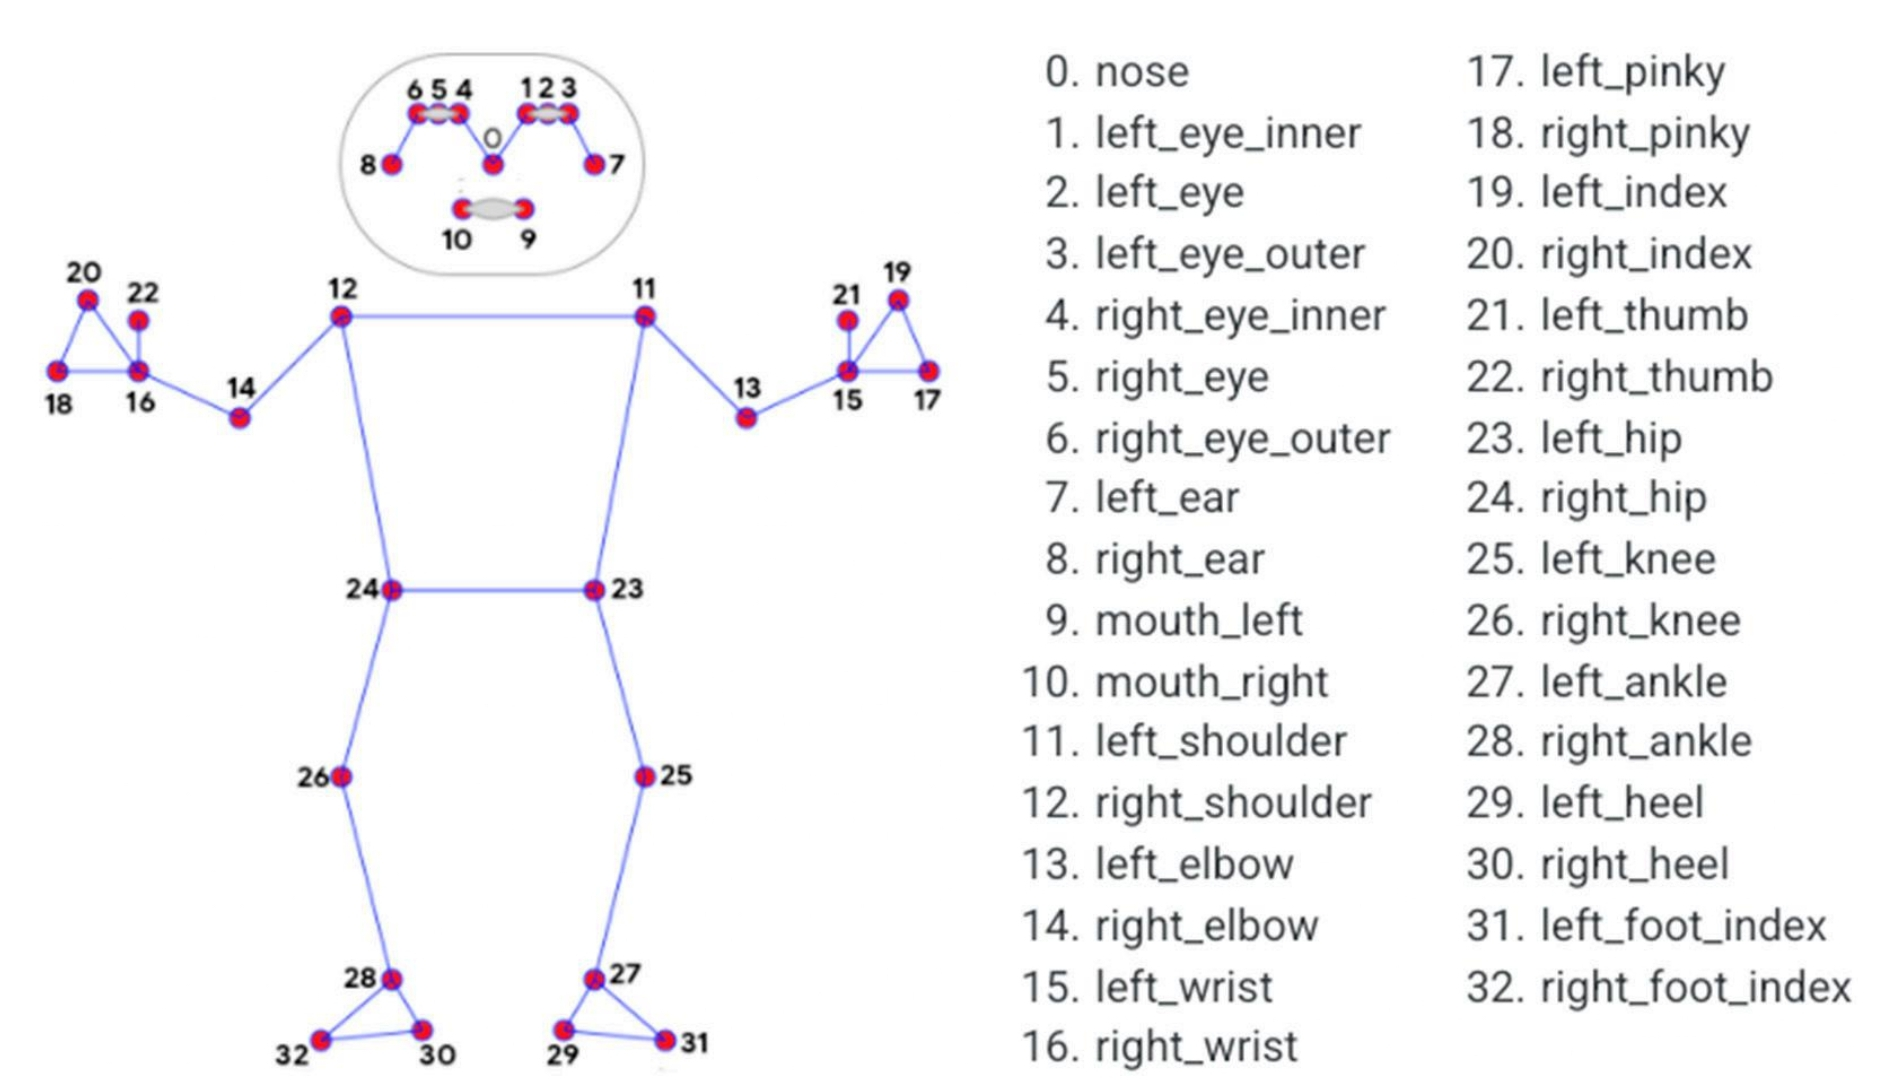
\includegraphics[scale=0.6]{gambar/mp_pose.jpg}

  % Ubah dengan keterangan gambar yang diinginkan
  \caption{Pose MediaPipe}
  \label{fig:Pose MediaPipe}
\end{figure}

\section{Classification Performance}
Dalam melakukan proses pengklasifikasian, diperlukan perhitungan efektifitas model yang telah dibuat berdasarkan beberapa pengukuran menggunakan set data pengetesan. Dalam hal ini, \emph{confusion matrix} merupakan salah satu perhitungan yang sering digunakan dalam kasus pengklasifikasian.

\emph{Confusion matrix} merupakan salah satu pengukuran yang paling mudah dilakukan dalam mencari nilai tingkat kebenaran dan juga akurasi dari model. \emph{Confusion matrix} adalah sebuah tabel berbentuk dua dimensi yang terdiri dari data aktual dan data prediksi yang masing-masing memiliki kelas. Data aktual terletak pada bagian kolom tabel, sedangkan data prediksi terletak pada bagian baris dari tabel. Gambar 2.3 merupakan representasi visual dari perhitungan confusion matrix.

% Contoh input gambar
\begin{figure}[H]
  \centering

  % Ubah dengan nama file gambar dan ukuran yang akan digunakan
  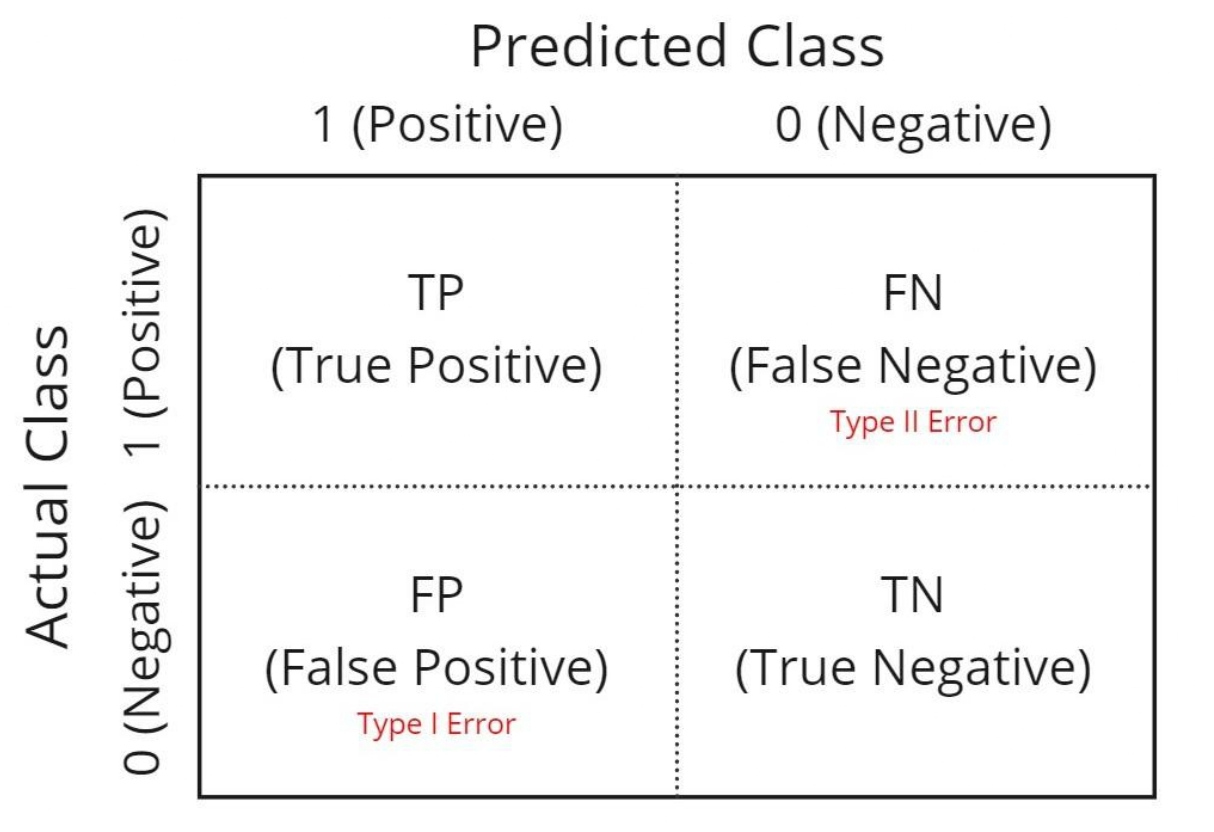
\includegraphics[scale=0.6]{gambar/halaman 37_page-0001 (1).jpg}

  % Ubah dengan keterangan gambar yang diinginkan
  \caption{Confusion Matrix}
  \label{fig:Confusion Matrix}
\end{figure}

\section{Evaluation Metrics}
\label{sec:gravitasi}
Penggunaan metrik evaluasi dalam konteks Deteksi Objek adalah sangat penting, karena ini berperan sebagai dasar kritis untuk membandingkan efektivitas berbagai algoritma dan skenario yang berbeda. Evaluasi yang teliti memungkinkan para peneliti untuk membuat perbandingan yang akurat antara berbagai teknik deteksi objek, serta menilai seberapa tepat tingkat keakuratan yang dicapai. Ini menjadi sangat vital dalam memilih algoritma yang paling cocok untuk tugas deteksi spesifik. Metrik seperti akurasi, presisi, dan recall adalah kunci dalam mengevaluasi seberapa efektif suatu model dalam mendeteksi dan mengidentifikasi objek dengan benar. Metrik-metrik ini penting untuk diimplementasikan demi menentukan model yang paling efisien.

Lebih lanjut, analisis akurasi memberikan wawasan kuantitatif yang signifikan mengenai kinerja algoritma deteksi objek, memberikan detail lebih lanjut mengenai kemampuan algoritma dalam menghasilkan deteksi yang akurat. Mengenali kesalahan melalui metrik evaluasi adalah langkah kritis dalam penelitian deteksi, seperti dalam kasus deteksi asap yang kami teliti. Langkah ini memfasilitasi identifikasi dan pemahaman tentang potensi kesalahan dalam algoritma, yang dapat membuka jalan untuk perbaikan dan peningkatan metode deteksi. Selanjutnya, metrik evaluasi juga mendukung pengoptimalan hiperparameter algoritma.

Dalam konteks penelitian ini, berbagai metrik evaluasi telah diterapkan, termasuk presisi, recall, dan Mean Average Precision (mAP). Dengan menggabungkan metode evaluasi ini, penelitian bertujuan untuk menyajikan analisis komprehensif mengenai kinerja dari algoritma deteksi objek yang ditinjau. Adapaun penjelasan konsep sederhana mengenai metrik evaluasi yang akan dijabarkan sebagai berikut :

\subsubsection*{1. Precision}
Precision merupakan rasio dimana TP (true positive) dimana jumlah positif benar dan FP (false positive) jumlah positif palsu sebagai metrik evaluasi dalam konteks machine learning, memberikan ukuran terhadap rasio prediksi positif yang tepat dibandingkan dengan seluruh prediksi positif yang diberikan oleh model. Dengan kata lain, precision 19 memberikan wawasan seberapa akurat model dalam membuat prediksi positif. Lebih rinci, precision mencerminkan seberapa sering model berhasil mengklasifikasikan instance sebagai positif dengan benar dalam keseluruhan dataset. Nilai precision dapat mengindikasikan sejauh mana model mampu memberikan prediksi yang benar dalam konteks positif. Rentang nilai precision berada antara 0 dan 1, di mana nilai 1 menunjukkan bahwa semua prediksi positif model adalah benar, sementara nilai 0 menunjukkan bahwa tidak ada prediksi positif yang benar.

\begin{equation}
    \frac{TP}{TP+FP}
\end{equation}

Pada persamaan diatas menyajikan perbandingan antara prediksi positif yang tepat dengan total prediksi positif yang diberikan oleh model, memberikan pandangan yang lebih mendalam terkait kemampuan model dalam menghasilkan hasil yang benar dalam kategori yang diinginkan

\subsubsection*{2. Recall}
Recall merupakan metrik yang digunakan untuk mengukur rasio dari data positif yangbenar yang ditemukan dari seluruh data positif. Recall memberikan informasi tentang seberapa baik model machine learning menemukan semua data positif. Nilai recall berkisar antara 0 dan 1. Recall yang tinggi menunjukan bahwa kelas yang dikenali dengan benar banyak, atau false negative yang didapatkan sedikit. Rumus dari recall dapat dilihat pada persamaan dibawah

\begin{equation}
    \frac{TP}{TP+FN}
\end{equation}

Recall merupakan rasio dimana TP (true positif ) adalah jumlah positif benar dan FN (false negative) jumlah negatif palsu

\subsubsection*{3. Mean Average Precision (mAP}
Mean Average Precision (mAP) adalah sebuah metrik akurasi yang dihasilkan dari menghitung rata-rata dari Average Precision (AP) atau presisi rata-rata. AP sendiri diperoleh melalui perhitungan precision dan recall. Oleh karena itu, mAP dapat dianggap sebagai metrik evaluasi yang sangat informatif dalam mengevaluasi kinerja suatu sistem.

\begin{equation}
    AP=\sum ((Recall_{n+1}-Recall_{n})\times Precision_{interp}\times Recall_{n+1})
\end{equation}
\begin{equation}
    mAP=\frac{1}{n}\sum_{n}^{i=1}AP_{i}
\end{equation}

\section{Intersection over Union (IoU)}
\label{subsec:hukumnewton}

Intersection over Union, atau IoU, adalah metrik yang digunakan untuk mengevaluasi keakuratan posisi objek yang dideteksi oleh model dalam pemrosesan gambar. Prinsipnya adalah dengan menghitung area persinggungan antara kotak deteksi yang dihasilkan oleh model dengan kotak referensi yang merupakan standar emas atau Ground Truth. Rasio ini didapat dengan membandingkan area irisan kedua kotak tersebut terhadap keseluruhan area yang mereka cakup secara bersamaan. Jika kita membayangkan kedua kotak tersebut sebagai satu kesatuan, maka IoU memberikan kita sebuah skor yang mengukur seberapa baik model kita dalam memprediksi lokasi objek sebenarnya. Semakin besar area persinggungan relatif terhadap total area gabungan, semakin tinggi nilai IoU, yang menandakan keakuratan prediksi yang lebih baik. Secara Sistematis, hal ini dituliskan sebagai :

% Contoh pembuatan persamaan
\begin{equation}
IntersectionoverUnion(IoU) = \frac{\left |A\bigcap B  \right |}{\left | A\bigcup B \right |}.
\end{equation}

IoU, atau Intersection over Union, merupakan metode penilaian yang mengukur efektivitas model deteksi objek dengan membandingkan area overlap antara prediksi model dan posisi objek aktual. Skala nilai IoU berada antara 0 hingga 1, di mana nilai yang lebih dekat ke 1 menandakan prediksi yang sangat akurat terhadap objek sebenarnya. Nilai IoU yang lebih tinggi menunjukkan bahwa model tersebut lebih tepat dalam mengidentifikasi dan menentukan lokasi objek.

Dalam skenario penelitian, misalnya pengenalan otomatis seekor hewan dalam sebuah gambar, model pembelajaran mendalam akan menciptakan sebuah kotak pembatas sebagai prediksi lokasi hewan tersebut. Kotak pembatas ini lalu dibandingkan dengan kotak kebenaran dasar—area yang telah ditentukan secara manual sebagai lokasi sebenarnya dari hewan dalam gambar. IoU kemudian dihitung untuk menilai seberapa baik kotak prediksi menutupi kotak kebenaran dasar, dengan mempertimbangkan area bersama dan area gabungan dari kedua kotak tersebut.

Dengan demikian, IoU berfungsi sebagai alat ukur yang penting dalam mengevaluasi kemampuan sebuah model deteksi objek untuk secara akurat menentukan posisi objek dalam berbagai kondisi, seperti variasi ukuran, orientasi, dan konteks objek dalam gambar. Sebuah nilai IoU yang tinggi menunjukkan bahwa model tersebut dapat diandalkan dalam mendeteksi dan mengidentifikasi objek dengan presisi yang tinggi.

\begin{figure}[H]
  \centering

  % Ubah dengan nama file gambar dan ukuran yang akan digunakan
  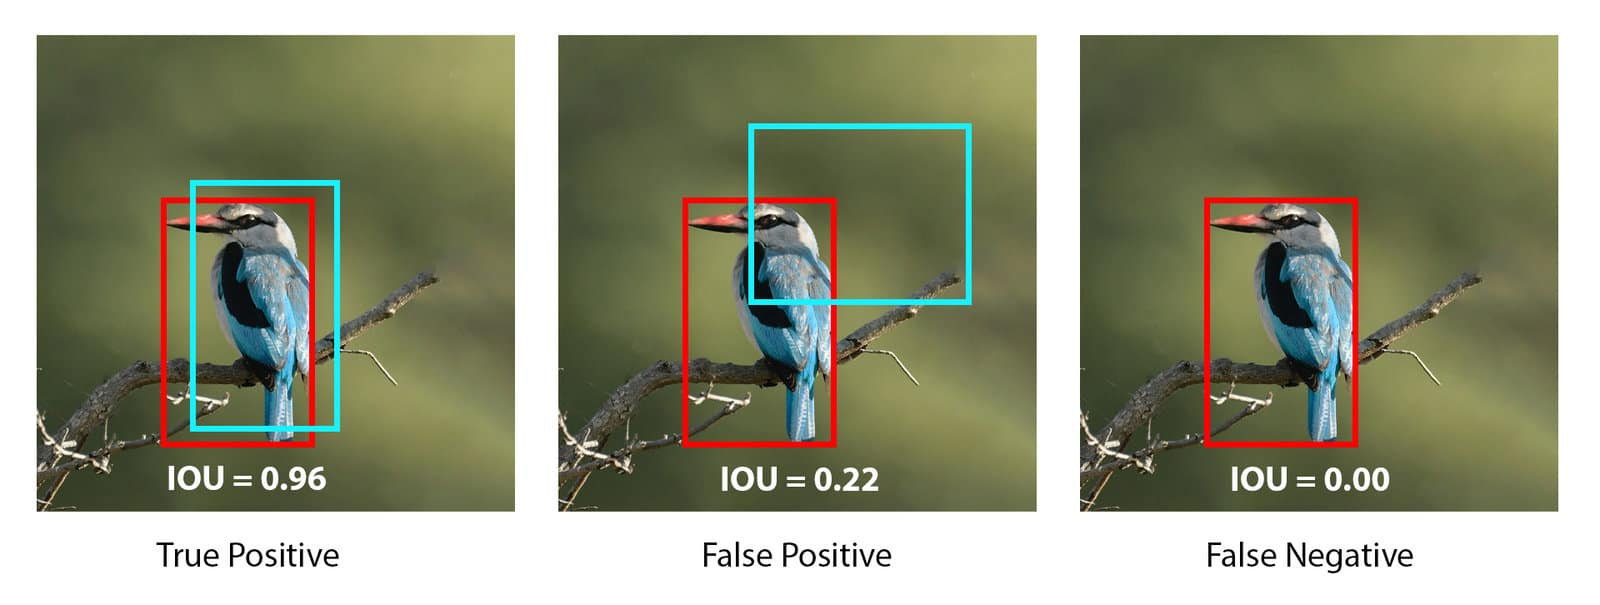
\includegraphics[scale=0.3]{gambar/Perbandingan nilai iou.jpg}

  % Ubah dengan keterangan gambar yang diinginkan
  \caption{Perbandingan Performa Berdasarkan IoU}
  \label{fig:roketluarangkasa}
\end{figure}

IoU menawarkan metode kuantitatif untuk mengevaluasi seberapa akurat model dalam mengenali dan menandai objek dalam gambar. Dalam proses pelatihan, nilai IoU minimal yang ditetapkan memungkinkan penetapan batas bagi kotak prediksi untuk dianggap cocok dengan deteksi yang benar, memfasilitasi penyesuaian antara tingkat akurasi deteksi dan insiden false positif. Penentuan batas IoU tidak bersifat tetap dan dapat disesuaikan, dengan 0,5 yang menjadi standar patokan awal. Kotak prediksi dengan IoU minimal 0,5 terhadap deteksi positif dianggap valid. Penyesuaian ambang nilai ini mempengaruhi balance antara presisi dan daya tangkap, dengan peningkatan nilai ambang cenderung mengurangi kesalahan positif namun berpotensi mengabaikan beberapa deteksi valid.

Penggunaan nilai kebenaran dasar dalam IoU merupakan perbandingan standar antara prediksi dan kondisi aktual objek yang diidentifikasi. Penandaan kotak kebenaran dasar, dilakukan secara manual oleh pakar, menentukan batas pasti objek dalam gambar. Skor IoU yang dihasilkan dari perbandingan antara prediksi model dengan batas ini memberikan wawasan terhadap efektivitas model dalam deteksi objek. Dataset kebenaran dasar, yang meliputi kotak pembatas yang ditandai secara manual, menjadi kunci dalam proses evaluasi ini, memberikan dasar objektif untuk mengukur kinerja algoritme deteksi objek.

Dengan demikian, IoU bukan hanya sekedar metrik evaluasi tetapi juga alat penting dalam pengembangan dan penyesuaian model deteksi objek, memastikan bahwa model dapat diandalkan dan akurat dalam berbagai kondisi dan skenario pengujian. \parencite{shah2023intersection}

\section{Single Board Computer (SBC)}
Single Board Computer (SBC) adalah komputer lengkap yang dibangun pada satu papan sirkuit tunggal, dengan mikroprosesor, memori, input/output (I/O), dan fitur lain yang diperlukan untuk fungsi komputer penuh. SBC dirancang untuk menjadi kompak dan efisien, sering digunakan dalam aplikasi tertanam, perangkat IoT, dan proyek-proyek pengembangan karena kemudahan penggunaan dan ukurannya yang kecil. SBC menyediakan platform yang ideal untuk pengembangan prototipe dan implementasi sistem kontrol dalam berbagai aplikasi, termasuk kursi roda otonom.

Dalam perkembangan teknologi , penggunaan Single Board Computer (SBC) seperti Intel NUC, NVIDIA Jetson Nano Developer Kit dan Rasberry Pi 4 telah berperan sangat penting terutama dalam Deteksi Real-time. Kecepatan yang ditawarkan SBC dalam memproses data dari sensor dan kamera  , serta menjalankan model visi komputer berbasis deep learning membuat alat ini menjadi standar dalam memilih alat untuk implementasi model Deteksi secara real time. Selain itu SBC juga biasanya dilengkapi dengan konektifitas yang sangat baik sehingga dapat terhubung dengan banyak IO. \parencite{Elliot_Residing}

\section{Roboflow}
RoboFlow adalah platform yang mendukung pengembangan dan penyebaran aplikasi visi komputer dengan menyediakan alat-alat canggih untuk manajemen dan peningkatan dataset. Platform ini dirancang untuk memudahkan pengolahan, analisis, dan augmentasi data visual, sehingga mempercepat siklus pengembangan dan peningkatan model pembelajaran mesin.

\begin{figure}[H]
  \centering

  % Ubah dengan nama file gambar dan ukuran yang akan digunakan
  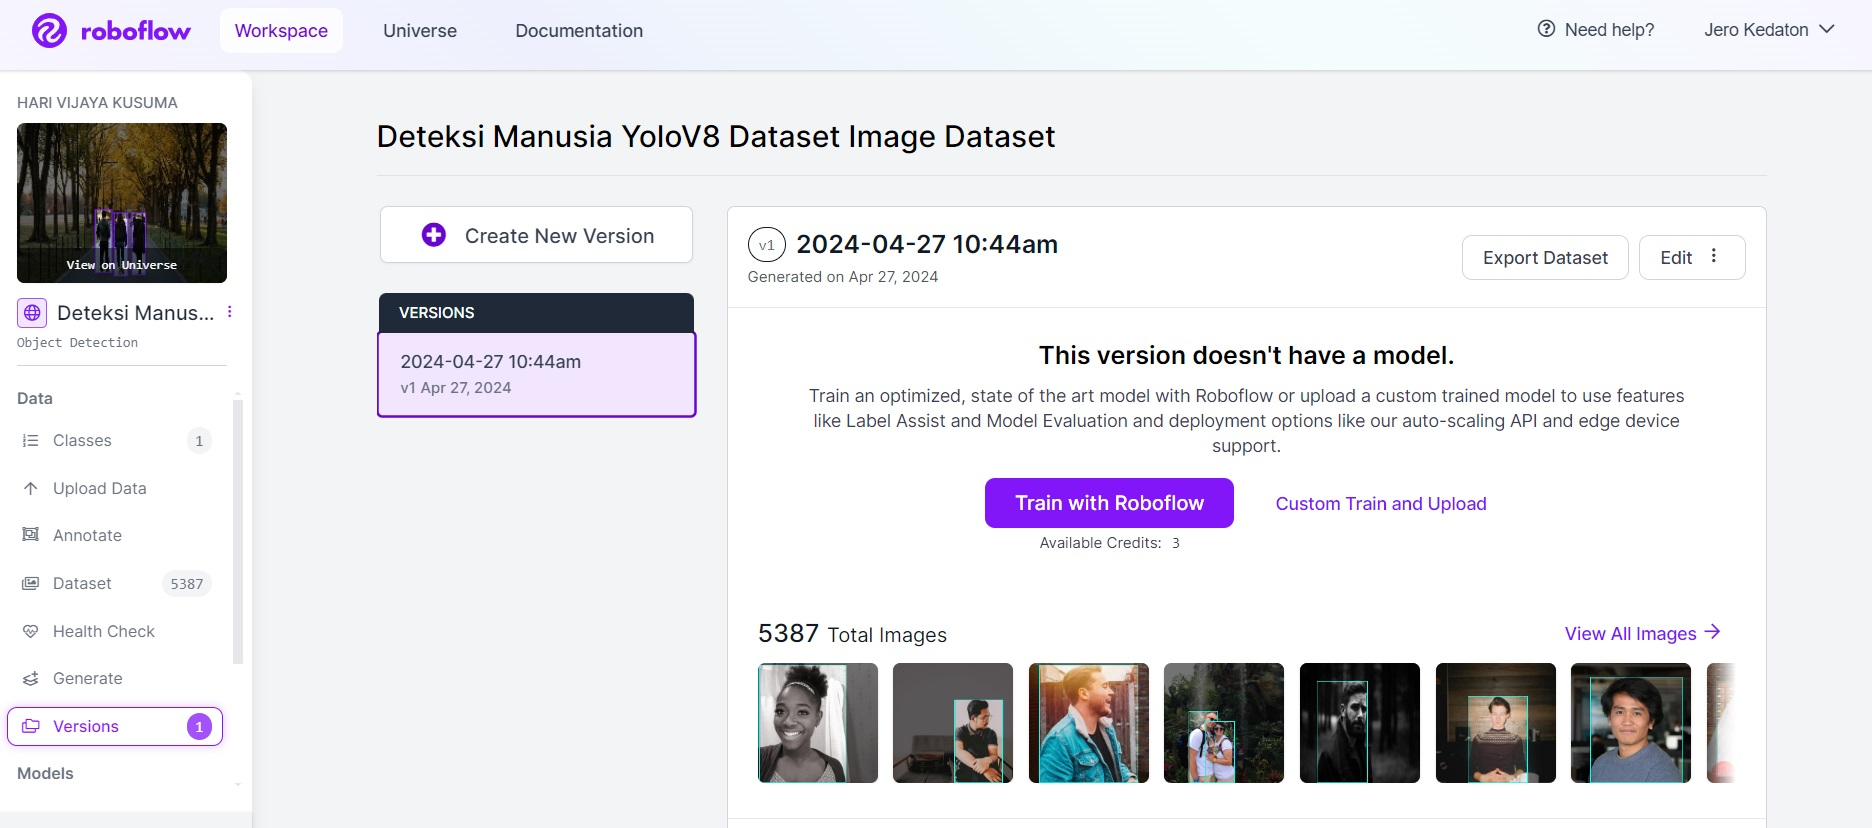
\includegraphics[scale=0.3]{gambar/roboflow.jpg}

  % Ubah dengan keterangan gambar yang diinginkan
  \caption{Interface Roboflow}
  \label{fig:roboflow}
\end{figure}

RoboFlow menyediakan serangkaian fungsi yang membantu dalam proses pengembangan model visi komputer, termasuk:
\begin{itemize}
    \item Annotasi Data : RoboFlow memungkinkan pengguna untuk menandai gambar dengan alat bantu yang intuitif, mempercepat proses pembuatan label untuk dataset.
    \item Augmentasi Data: Melalui augmentasi data, RoboFlow dapat secara otomatis memodifikasi gambar dalam dataset untuk menciptakan variasi, yang membantu dalam meningkatkan robustness model yang dilatih.
    \item Konversi Format Data: Platform ini mendukung konversi antara berbagai format dataset yang populer, memudahkan pengguna dalam mempersiapkan data untuk berbagai jenis algoritma pembelajaran mesin.
    \item Pemisahan Dataset: RoboFlow menyediakan fungsi untuk membagi dataset menjadi set pelatihan, validasi, dan pengujian, yang merupakan langkah penting dalam validasi model.
\end{itemize}
RoboFlow menawarkan integrasi yang mulus dengan banyak kerangka kerja pembelajaran mesin populer seperti TensorFlow, PyTorch, dan YOLO. Integrasi ini memungkinkan pengembang:
\begin{itemize}
    \item Ekspor Data: Pengguna dapat dengan mudah mengekspor dataset mereka dalam format yang siap digunakan oleh kerangka kerja pembelajaran mesin pilihan mereka.
    \item Pelatihan Model: Platform ini menyediakan alat yang memungkinkan pengguna untuk langsung melatih model mereka menggunakan dataset yang telah disiapkan dan dioptimalkan.
    \item Evaluasi Model: RoboFlow menyediakan metrik untuk mengukur kinerja model, membantu pengguna memahami efektivitas model mereka dan membuat penyesuaian yang diperlukan.
\end{itemize}

\section{Intel NUC}
Intel NUC (Next Unit of Computing) adalah solusi komputasi yang kompak dan kuat yang dirancang oleh Intel untuk memenuhi berbagai kebutuhan komputasi, mulai dari hiburan rumah hingga gaming dan tugas profesional. Intel NUC dengan fitur prosesor Intel Core generasi dalam form factor kompak 4x4 inci. Dirancang untuk menawarkan kombinasi ukuran, kinerja, keberlanjutan, dan keandalan yang dibutuhkan oleh bisnis modern. Intel NCU model tertentu juga menyertakan teknologi Intel vPro® Enterprise dengan keamanan yang ditingkatkan. Mini PC ini dapat diupgrade dan diperbaiki, menjadikannya pilihan serbaguna untuk berbagai aplikasi bisnis termasuk komputasi klien, komputasi edge, dan digital singage.

\begin{figure}[H]
  \centering

  % Ubah dengan nama file gambar dan ukuran yang akan digunakan
  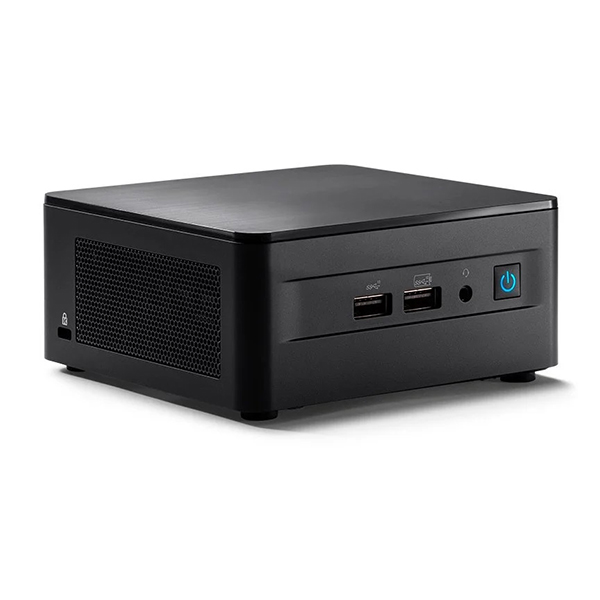
\includegraphics[scale=0.3]{gambar/INTEL-NUC-RNUC12WSHI30000-1.jpg}

  % Ubah dengan keterangan gambar yang diinginkan
  \caption{Gambar Intel NUC}
  \label{fig:roketluarangkasa}
\end{figure}

\section{ESP32 Devkit V1}

ESP32 Devkit V1 adalah salah satu development board yang dibuat oleh DOIT untuk menjalankan modul ESP-WROOM-32 buatan Espressif. ESP32 Devkit dikenal dengan Development board yang kaya fitur dengan konektivitas Wi-Fi dan Bluetooth terintegrasi untuk beragam aplikasi. Devkit ini memiliki banyak pin yang memungkinkannya untuk diprogram dengan banyak tugas.

\begin{figure}[H]
  \centering

  % Ubah dengan nama file gambar dan ukuran yang akan digunakan
  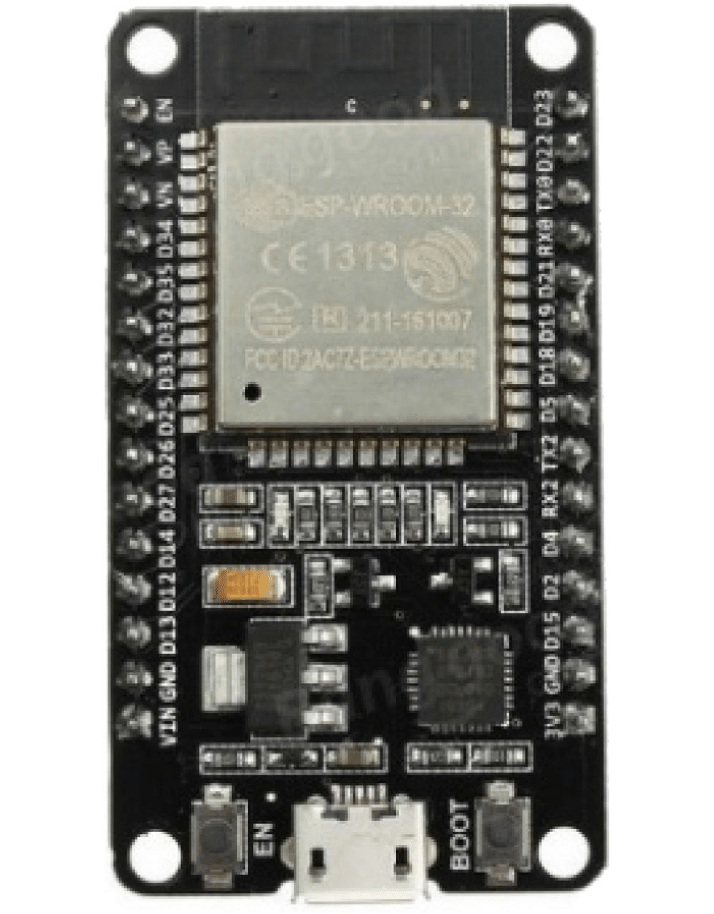
\includegraphics[scale=0.2]{gambar/The-ESP32-DEVKIT-V1-board-used-as-controller.png}

  % Ubah dengan keterangan gambar yang diinginkan
  \caption{Gambar ESP32 Devkit V1}
  \label{fig:roketluarangkasa}
\end{figure}

\section{Motor Driver H-Bridge}

Driver motor H-Bridge adalah rangkaian elektronik yang digunakan untuk mengontrol arah dan kecepatan motor DC. Cara kerjanya berdasarkan empat switch yang membentuk jembatan H (H-Bridge), yang mana dengan mengatur pembukaan dan penutupan switch-switch ini, kita dapat mengatur arah arus yang mengalir ke motor. Dengan demikian, kita bisa mengubah arah putaran motor DC. Driver Motor H-Bridge tersusun oleh sekumpulan transistor yang berfungsi sebagai pengendali motor, terutama yang memerlukan arus serta tegangan yang cukup besar. selain itu, Rangkaian H-Bridge juga dapat memberikan fungsi pengereman pada motor dengan menghubungkan kedua terminal motor sehingga motor dapat berhenti lebih cepat. \parencite{fibrianianalisis}

\begin{figure}[H]
  \centering

  % Ubah dengan nama file gambar dan ukuran yang akan digunakan
  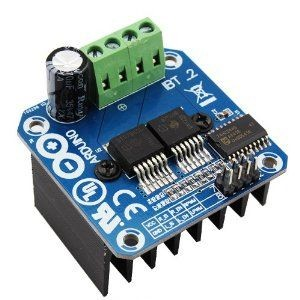
\includegraphics[scale=0.3]{gambar/Motor Driver H - bridge Bts.jpg}

  % Ubah dengan keterangan gambar yang diinginkan
  \caption{Gambar Motor Driver H-Bridge}
  \label{fig:roketluarangkasa}
\end{figure}

\section{Kursi Roda Elektrik KY-123}

Kursi roda bertenaga listrik merupakan alat bantu mobilitas yang terdiri dari struktur dasar kursi roda, sistem pengendalian gerak, mesin elektrik, dan modul baterai. Keunggulan alat ini terletak pada kemampuannya untuk dikendalikan dengan mudah dan nyaman, meminimalkan usaha fisik yang diperlukan pengguna dibandingkan dengan kursi roda manual. Ini sangat bermanfaat bagi individu dengan kondisi hemiplegia, memungkinkan pengoperasian dengan satu tangan. Selain itu, kursi roda elektrik ini juga memberikan solusi mobilitas yang lebih baik bagi lansia yang mengalami keterbatasan dalam bergerak.

\begin{figure}[H]
  \centering

  % Ubah dengan nama file gambar dan ukuran yang akan digunakan
  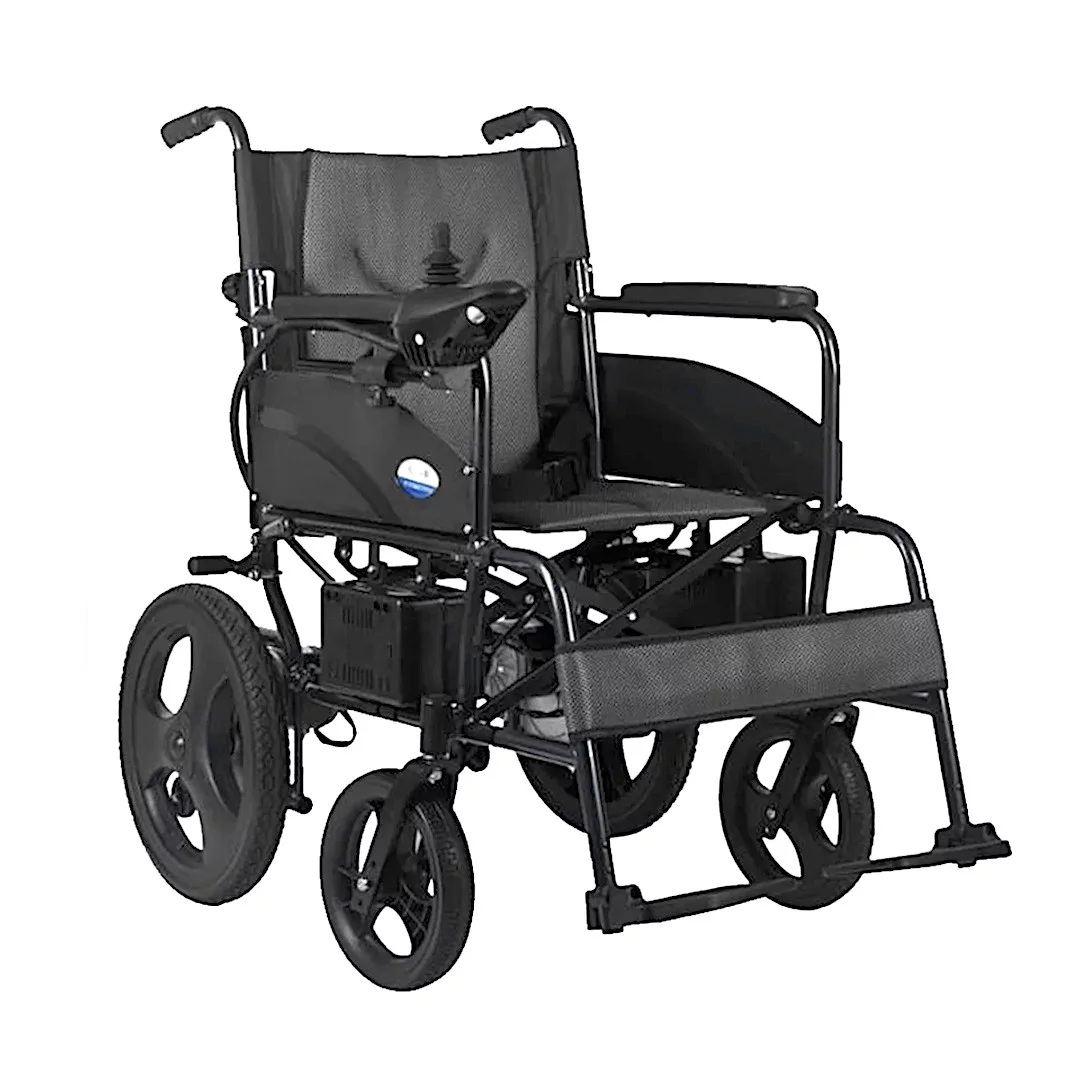
\includegraphics[scale=0.3]{gambar/Kursi Roda Elektrik Lipat OneHealth KY123 A.jpg}

  % Ubah dengan keterangan gambar yang diinginkan
  \caption{Gambar Kursi Roda Elektrik KY-123}
  \label{fig:roketluarangkasa}
\end{figure}

